% !TEX root = ../main.tex
\begin{figure}[tp]
\centering
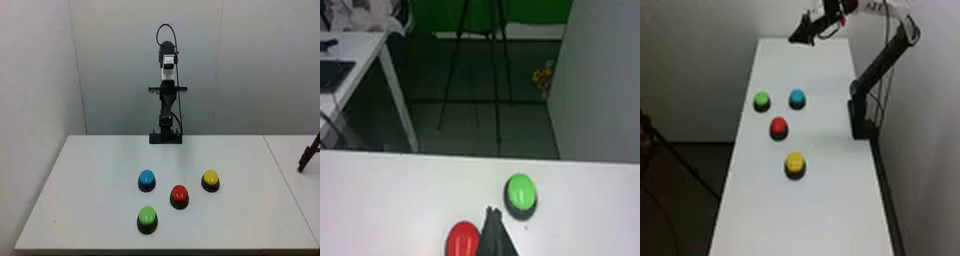
\includegraphics[width=0.8\linewidth]{figures/table30_subtask_keyframes_train/press_the_button/init.png}
\par\smallskip{\footnotesize\textbf{Stage 1.} Press the pink button.\par}
\medskip
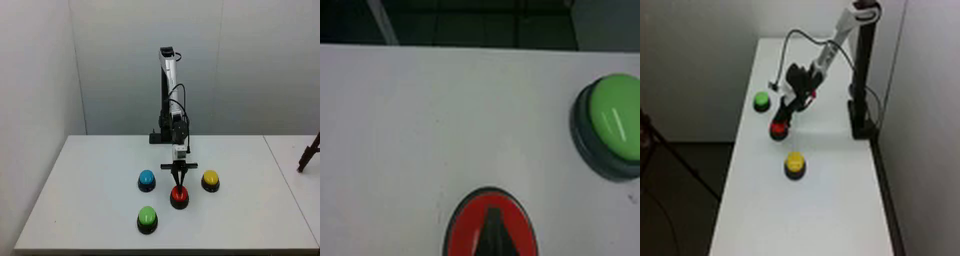
\includegraphics[width=0.8\linewidth]{figures/table30_subtask_keyframes_train/press_the_button/01_press_2.png}
\par\smallskip{\footnotesize\textbf{Stage 2.} Press the blue button.\par}
\medskip
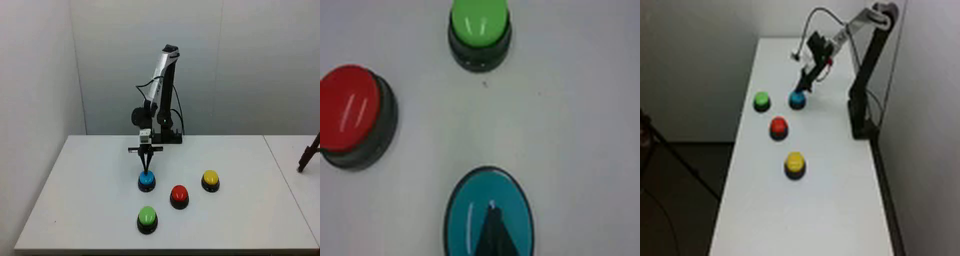
\includegraphics[width=0.8\linewidth]{figures/table30_subtask_keyframes_train/press_the_button/02_press_3.png}
\par\smallskip{\footnotesize\textbf{Stage 3.} Press the green button.\par}
\medskip
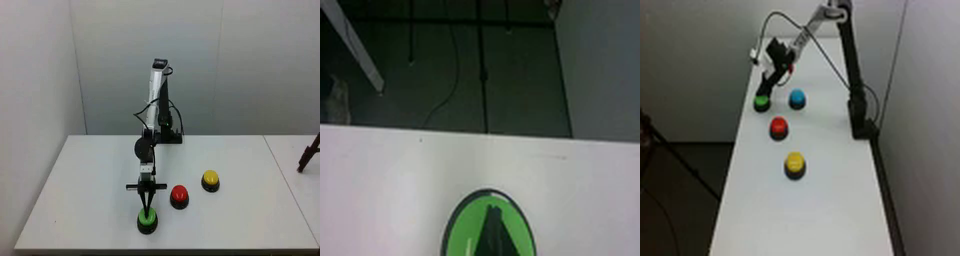
\includegraphics[width=0.8\linewidth]{figures/table30_subtask_keyframes_train/press_the_button/03_press_4.png}
\par\smallskip{\footnotesize\textbf{Stage 4.} Press the yellow button, then retract the gripper.\par}
\caption{\textbf{Button pressing (ARX5).} Subtask segmentation example. The initial observation (Stage 1) and subsequent stage observations are shown in order, each paired with its subtask instruction.}
\label{fig:subtask_press_the_button}
\end{figure}

\begin{figure}[tp]
\centering
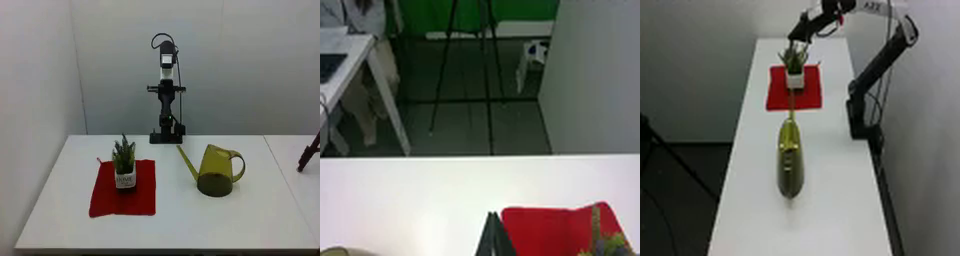
\includegraphics[width=0.8\linewidth]{figures/table30_subtask_keyframes_train/water_the_flowers/init.png}
\par\smallskip{\footnotesize\textbf{Stage 1.} Pick up the watering can and water the potted plant.\par}
\medskip
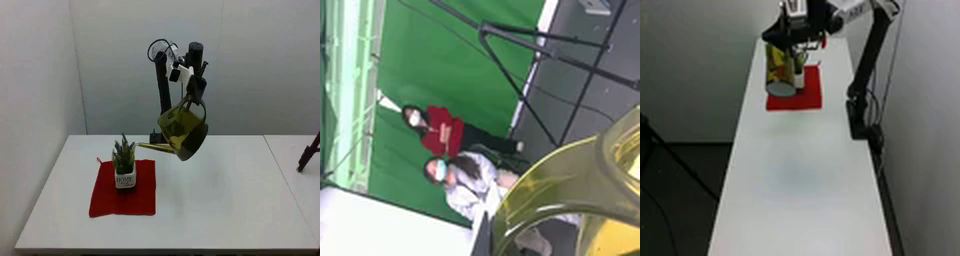
\includegraphics[width=0.8\linewidth]{figures/table30_subtask_keyframes_train/water_the_flowers/01_place.png}
\par\smallskip{\footnotesize\textbf{Stage 2.} The watering is finished, put the watering can down.\par}
\caption{\textbf{Plant watering (ARX5).} Subtask segmentation example. The initial observation (Stage 1) and subsequent stage observations are shown in order, each paired with its subtask instruction.}
\label{fig:subtask_water_the_flowers}
\end{figure}

\begin{figure}[tp]
\centering
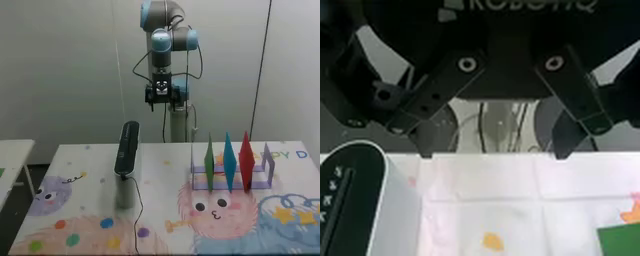
\includegraphics[width=0.8\linewidth]{figures/table30_subtask_keyframes_train/shred_paper/init.png}
\par\smallskip{\footnotesize\textbf{Stage 1.} Put the paper into the shredder.\par}
\medskip
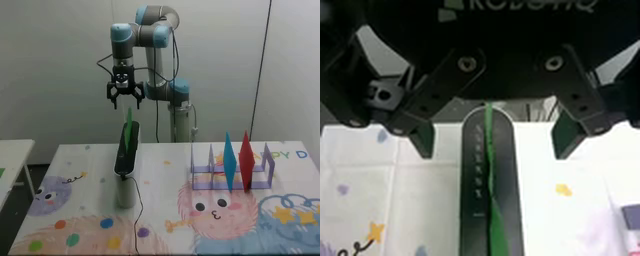
\includegraphics[width=0.8\linewidth]{figures/table30_subtask_keyframes_train/shred_paper/01_retract.png}
\par\smallskip{\footnotesize\textbf{Stage 2.} Retract gripper.\par}
\caption{\textbf{Paper shredding (UR5).} Subtask segmentation example. The initial observation (Stage 1) and subsequent stage observations are shown in order, each paired with its subtask instruction.}
\label{fig:subtask_shred_paper}
\end{figure}

\begin{figure}[tp]
\centering
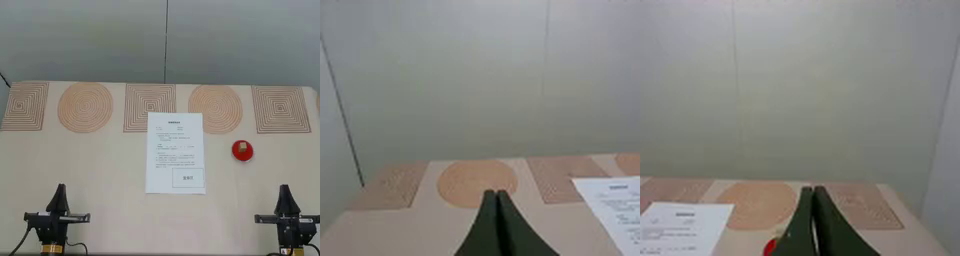
\includegraphics[width=0.8\linewidth]{figures/table30_subtask_keyframes_train/stamp_positioning/init.png}
\par\smallskip{\footnotesize\textbf{Stage 1.} Pick up the stamp.\par}
\medskip
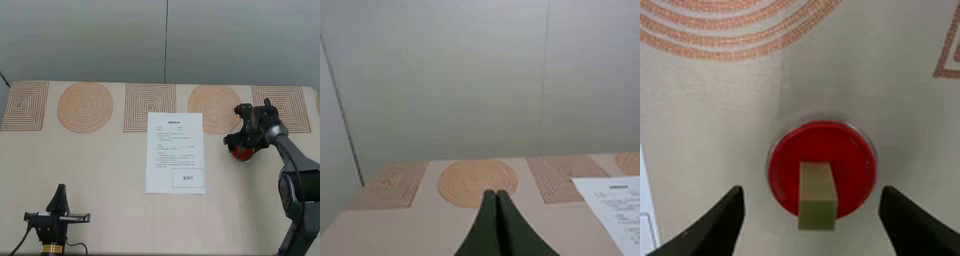
\includegraphics[width=0.8\linewidth]{figures/table30_subtask_keyframes_train/stamp_positioning/01_dip.png}
\par\smallskip{\footnotesize\textbf{Stage 2.} Dip into the ink.\par}
\medskip
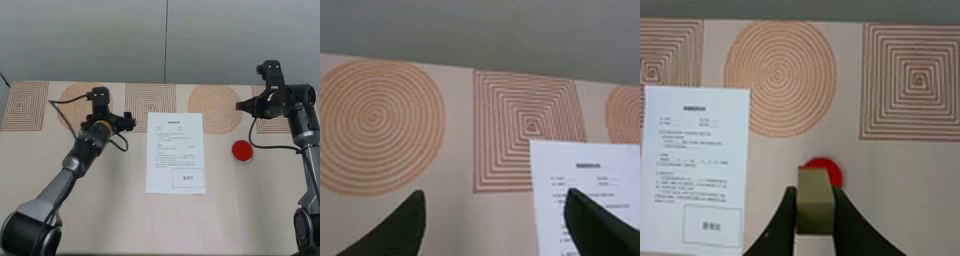
\includegraphics[width=0.8\linewidth]{figures/table30_subtask_keyframes_train/stamp_positioning/02_stamp.png}
\par\smallskip{\footnotesize\textbf{Stage 3.} Stamp the signature area and return.\par}
\caption{\textbf{Stamp positioning (ALOHA).} Subtask segmentation example. The initial observation (Stage 1) and subsequent stage observations are shown in order, each paired with its subtask instruction.}
\label{fig:subtask_stamp_positioning}
\end{figure}
